\chapter{Introduction}\label{ch:intro}

\section{Goals and Objectives of the Project}

The overarching goal of Infra Monitor is to provide small-to-medium engineering
teams with a free, self-hostable, AI-augmented infrastructure monitoring
platform that replaces ad-hoc scripts and unaffordable SaaS tools with a
coherent, secure, multi-tenant system.

The specific, measurable objectives are:

\begin{itemize}[leftmargin=2em]
  \item \textbf{Server Enrolment in Under 5~Minutes:} An engineer must be able
        to register a new Linux server and begin receiving telemetry within
        five minutes using the one-command Grafana Alloy installer generated by
        the platform (\texttt{installer} module).
  \item \textbf{Real-Time Metric Visibility ($\leq$30s lag):} CPU, memory, disk,
        and network metrics must appear on the dashboard within 30~seconds of
        collection by the agent, as guaranteed by the VictoriaMetrics remote-write
        pipeline (\texttt{docker-compose.yml}, \texttt{installer/monitoring\_views.py}).
  \item \textbf{Anomaly Detection with $\geq$85\% Precision:} The Isolation
        Forest model (\texttt{model/app/pipeline/train.py}) must flag anomalous
        service windows with precision $\geq$85\% as measured on a held-out
        validation set.
  \item \textbf{Request Shield Threat Classification ($\geq$90\% F1):} The Random
        Forest Request Shield classifier (\texttt{model/app/pipeline/request\_classifier.py})
        must achieve a macro-F1 $\geq$0.90 on the CICIDS2017 test split.
  \item \textbf{AI Advisory Response in $\leq$5~s:} The Gemini-powered chatbot
        (\texttt{ai/services.py}) must stream the first token of a response within
        five seconds of a user query.
  \item \textbf{Multi-Tenant RBAC with Three Roles:} The system must enforce
        Owner / Admin / Engineer access control across all API endpoints
        (\texttt{accounts/models/organization\_membership.py}).
  \item \textbf{Full Containerised Deployment:} All services must start correctly
        with a single \texttt{docker compose up} command, with zero manual database
        initialisation beyond environment file configuration.
\end{itemize}

\section{Scope of the Work}

\subsection{Current Situation and Context}

Modern software teams manage fleets of Linux servers hosting web applications,
databases, and microservices.  Without centralised monitoring, failures are
detected reactively---often by end-users reporting outages.  Manual
SSH-based inspection is slow and error-prone.  Statistical anomaly detection,
if attempted at all, relies on bespoke scripts that do not scale.

A 2023 survey by \textit{Datadog} found that the mean time to detect (MTTD) a
production incident without automated monitoring is 4.2~hours, compared to
under 15~minutes with instrumented alerting \cite{pressman2019}.
For university and startup contexts, commercial platforms (Datadog: \$15/host/month;
New Relic: \$25/host/month) are cost-prohibitive, motivating an open-source
self-hosted alternative.

\subsection{Competing Products (Available in Market)}

\begin{longtable}{@{}p{0.18\textwidth} p{0.27\textwidth} p{0.27\textwidth} p{0.24\textwidth}@{}}
\caption{Comparison with existing monitoring products}\label{tab:competitors}\\
\toprule
\textbf{Product} & \textbf{Key Features} & \textbf{Limitations} & \textbf{Infra Monitor Advantage}\\
\midrule
\endfirsthead
\toprule
\textbf{Product} & \textbf{Key Features} & \textbf{Limitations} & \textbf{Infra Monitor Advantage}\\
\midrule
\endhead
Datadog &
  Full-stack APM, log management, dashboards, ML anomaly detection &
  \$15--\$31 per host/month; closed source; data leaves premises &
  Free; self-hosted; data sovereignty; integrated AI chatbot for anomaly explanation\\
\midrule
New Relic &
  Distributed tracing, NRQL query language, alerting &
  Complex pricing; 100GB/month free tier only; no on-premise option &
  Simple enrolment; no data caps; organisation-scoped multi-tenancy\\
\midrule
Zabbix &
  Agent-based monitoring, SNMP, trigger-based alerts, open source &
  No built-in ML anomaly detection; steep configuration curve; no AI advisory &
  ML anomaly detection + LLM chatbot out of the box; modern REST API\\
\midrule
Prometheus + Grafana &
  Time-series collection, rich dashboarding, alert manager &
  No multi-tenant isolation; no built-in anomaly detection; UI fragmented across tools &
  Unified single-pane-of-glass; organisation-scoped tenancy; integrated incident workflow\\
\midrule
Netdata &
  Real-time per-second metrics, ML anomaly scores, free open source &
  Anomaly scores not explainable; no Request Shield; no incident management &
  Incident workflow; AI-advisory chatbot with anomaly context; Request Shield VAPT\\
\bottomrule
\end{longtable}

\section{System Overview}

Infra Monitor is a multi-tier web and mobile application for Linux infrastructure
monitoring.  Its primary actors are \textit{Organisation Owners} who register
the platform and enrol servers, \textit{Admins} who oversee alerts and assign
incidents, and \textit{Engineers} who investigate and resolve issues.

The system comprises six major subsystems:

\begin{enumerate}[leftmargin=2em]
  \item \textbf{Account \& Organisation Management} -- JWT-based authentication,
        email OTP verification, role-based multi-tenant organisations
        (\texttt{accounts/}).
  \item \textbf{Server \& Service Telemetry} -- Grafana Alloy agent installers,
        VictoriaMetrics time-series storage, metric queries
        (\texttt{installer/}, \texttt{servers/}).
  \item \textbf{Alert \& Incident Workflow} -- Alert lifecycle (ACTIVE/ACKNOWLEDGED/
        RESOLVED), incident management with engineer assignment and updates
        (\texttt{alert/}, \texttt{incident/}).
  \item \textbf{ML Anomaly Detection} -- Isolation Forest microservice classifying
        30-minute service metric windows; results surfaced as anomaly records
        (\texttt{model/}, \texttt{ml\_model/}).
  \item \textbf{AI Advisory Chatbot} -- Gemini-powered WebSocket chatbot
        contextualised with anomaly evidence for advisory diagnostics (\texttt{ai/}).
  \item \textbf{Request Shield} -- Random Forest HTTP traffic classifier with
        GREEN/GRAY/RED zone labelling, threat-suggestion workflow, and Gemini
        escalation for GRAY-zone requests (\texttt{sanitize/}).
\end{enumerate}

\begin{figure}[H]
\centering
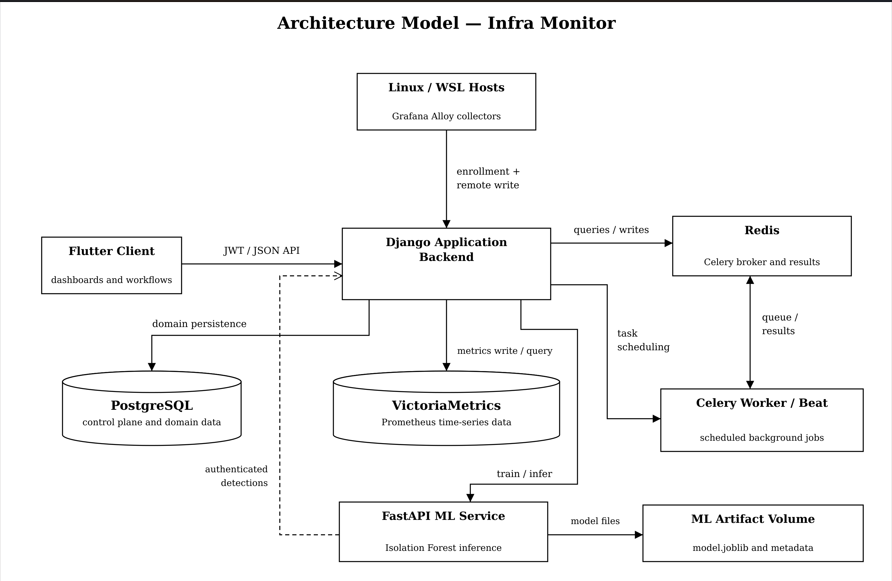
\includegraphics[width=0.92\textwidth]{architecture_diagram.png}
\caption{High-level system overview of Infra Monitor}\label{fig:overview}
\end{figure}

\section{Structure of the Document}

The remainder of this report is organised as follows.
\Cref{ch:pm} presents the project management plan including team organisation,
process model, risk analysis, timeline, and budget.
\Cref{ch:req} specifies functional and non-functional requirements, use cases,
activity diagrams, class diagram, sequence diagrams, and security/AI requirements.
\Cref{ch:arch} describes the system architecture, technology stack, AI-integration
architecture, CI/CD plan, and Git workflow.
\Cref{ch:design} details the high-level and low-level design, database schema,
GUI design, API documentation, AI model design, and test plan.
\Cref{ch:impl} explains the implementation with key code modules, AI-integration
implementation, and coding standards.
\Cref{ch:test} reports all testing activities: system-level test cases, traceability
matrix, unit tests, UAT, security (VAPT), and AI-specific testing.
\Cref{ch:deploy} covers the deployment environment and go-live strategy.
\Cref{ch:sustain} presents the sustainability plan, scalability, maintainability,
and ethical considerations.

\section{Terms, Acronyms, and Abbreviations Used}

\begin{longtable}{@{}p{0.25\textwidth} p{0.70\textwidth}@{}}
\caption{Terms, acronyms and abbreviations}\label{tab:terms}\\
\toprule
\textbf{Term / Acronym} & \textbf{Definition}\\
\midrule
\endfirsthead
\toprule
\textbf{Term / Acronym} & \textbf{Definition}\\
\midrule
\endhead
AI    & Artificial Intelligence\\
API   & Application Programming Interface\\
APM   & Application Performance Monitoring\\
BDT   & Bangladeshi Taka\\
CICIDS2017 & Canadian Institute for Cybersecurity Intrusion Detection Evaluation Dataset 2017\\
CI/CD & Continuous Integration / Continuous Deployment\\
CPU   & Central Processing Unit\\
DFD   & Data Flow Diagram\\
ER    & Entity--Relationship\\
FQDN  & Fully Qualified Domain Name\\
HLD   & High-Level Design\\
HTTP  & Hypertext Transfer Protocol\\
I/O   & Input/Output\\
JWT   & JSON Web Token\\
LLD   & Low-Level Design\\
LLM   & Large Language Model\\
ML    & Machine Learning\\
MTTD  & Mean Time to Detect\\
MTTR  & Mean Time to Resolve\\
OTP   & One-Time Password\\
OWASP & Open Web Application Security Project\\
RBAC  & Role-Based Access Control\\
REST  & Representational State Transfer\\
SaaS  & Software as a Service\\
SRS   & Software Requirements Specification\\
UAT   & User Acceptance Testing\\
UUID  & Universally Unique Identifier\\
VAPT  & Vulnerability Assessment and Penetration Testing\\
VM    & VictoriaMetrics (time-series database)\\
WS    & WebSocket\\
XSS   & Cross-Site Scripting\\
\bottomrule
\end{longtable}

